\documentclass[sigconf]{acmart}
\usepackage{polyglossia}
\usepackage{booktabs} % For formal tables


% Copyright
%\setcopyright{none}
\setcopyright{acmcopyright}
%\setcopyright{acmlicensed}
%\setcopyright{rightsretained}
%\setcopyright{usgov}
%\setcopyright{usgovmixed}
%\setcopyright{cagov}
%\setcopyright{cagovmixed}


\begin{document}
\title{SIG Proceedings Paper in LaTeX Format}
\titlenote{Produces the permission block, and
  copyright information}
\subtitle{Extended Abstract}
\subtitlenote{The full version of the author's guide is available as
  \texttt{acmart.pdf} document}


\begin{abstract}
This paper provides a sample of a \LaTeX\ document which conforms,
somewhat loosely, to the formatting guidelines for
ACM SIG Proceedings.\footnote{This is an abstract footnote}
\end{abstract}

%
% The code below should be generated by the tool at
% http://dl.acm.org/ccs.cfm
% Please copy and paste the code instead of the example below.
%
\begin{CCSXML}
<ccs2012>
 <concept>
  <concept_id>10010520.10010553.10010562</concept_id>
  <concept_desc>Computer systems organization~Embedded systems</concept_desc>
  <concept_significance>500</concept_significance>
 </concept>
 <concept>
  <concept_id>10010520.10010575.10010755</concept_id>
  <concept_desc>Computer systems organization~Redundancy</concept_desc>
  <concept_significance>300</concept_significance>
 </concept>
 <concept>
  <concept_id>10010520.10010553.10010554</concept_id>
  <concept_desc>Computer systems organization~Robotics</concept_desc>
  <concept_significance>100</concept_significance>
 </concept>
 <concept>
  <concept_id>10003033.10003083.10003095</concept_id>
  <concept_desc>Networks~Network reliability</concept_desc>
  <concept_significance>100</concept_significance>
 </concept>
</ccs2012>
\end{CCSXML}

\ccsdesc[500]{Computer systems organization~Embedded systems}
\ccsdesc[300]{Computer systems organization~Redundancy}
\ccsdesc{Computer systems organization~Robotics}
\ccsdesc[100]{Networks~Network reliability}


\keywords{ACM proceedings, \LaTeX, text tagging}


\maketitle

\section{Introduction}
As humans and robots start working in closer proximity to each other, it becomes vital that we design robot communication strategies which closely match human expectations. Body language plays a key role in how humans communicate with each other \cite{mcneill:levine} and we hypothesize that enabling robots to exhibit human-like body language while engaging in conversation will make them seem more engaging, friendly, and relatable.

Our work explores the design, implementation, and evaluation of a non-realtime system to generate body language for robots. Gestures can be classified into four types: metaphorics, iconics, deictics, and beats \cite{mcneill:levine}. We focus specifically on beat gestures, which are rhythmic, repetitive motions that humans use to emphasize key phrases. Specifically, we want to test the role of prosody- and emotion-based beat gestures in conveying emphasis, emotion, and personality in solo robot performances, accompanied by human speech.

Prosody features are known to correspond well to emphasis in speech \cite{terken:levine}. Likewise, beat gestures are also consistent with emphasis \cite{mcneill:levine}. Additionally, humans tend to express emotion physically which reinforces the content of their speech \cite{vosk}. Doing sentiment analysis on the content of the spoken word should therefore allow us to extract points of emotional emphasis in human speech and generate gestures to accompany this emphasis.

Specifically, our contributions are threefold: 1) building a system that generates gestures based on the prosody and emotional features of accompanying speech, 2) designing a mapping from human joint positions to robot joint positions and, 3) subjectively evaluating the effectiveness of robot body language. Our informal subjective evaluation provides mixed evidence for our hypothesis that prosody- and emotion-driven synthesis generate the most human-like gestures.

\section{Related Work}
As interaction between humans and robots becomes more commonplace, we must design robots behaviors such that they conform to what humans expect out of a one-to-one interaction. Saleh et al \cite{saleh:10} show how robots can benefit from reading a human\textquotesingle s facial expressions and understanding the true intent behind a human\textquotesingle s utterances. Having said that, communication is a two-way street and we are interested in solving the complementary problem.

Body language plays a key role in how human beings communicate with each other. Specifically, physical gestures supplement speech and therefore, are vital elements in the vocabulary of human communication. In order to make robots more relatable and to create a feeling of natural affinity between robots and humans, it is important that robots become capable of supplementing their speech with gestures.

Breazeal et al \cite{breazeal:8} show that humans are consistently able to infer mental states of a robot via both explicit and implicit behaviors. This reveals the idea that humans have strong expectations regarding how nonverbal cues map to mental states and therefore shows that such cues are vital to productive human-robot interaction.

Like \cite{breazeal:8}, Admoni et al \cite{admoni:7} develop nonverbal actions (via gaze manipulation) based on the current context, human intentions, and perception within an interactive environment. This addresses only a small part of nonverbal interaction problem. For instance, a person who is happy will be more active and energetic with full-body motions than a person who is sad. We intend to communicate emotion and affect through full-body motions, keeping in mind the current context and perception.

Physical gestures can be divided into 4 categories according to \cite{mcneill:levine}. We intend to focus on beat gestures in our work for programmatic ease. Beat gestures are rhythmic hand motions that can convey emotion and personality. One can imagine the use of such gestures by presenters or tour guides to convey a feeling of excitement or to emphasize a certain point.

There are a number of approaches presented in the literature concerning gesture modeling. However, most existing methods are used to generate animation sequences (from spoken words) for virtual characters. Levine et al \cite{levine:2} provide a framework for generating full-body animations from live speech. This involves designing a predictive model based on prosody (pitch, intensity, duration) features. The model itself is a Hidden Markov Model and the training phase does not require any hand-labeling of input data.

This approach, however, is limited by the features being used, i.e., prosody. For instance, two people, speaking very loudly, could have the same prosody features, but one person could be speaking in an excited manner upon seeing an old friend, and another in an angry way. So we must also incorporate emotion features tied with the words being spoken. DeepMoji \cite{deepmojipaper:3} goes beyond the binary positive/negative sentiment analysis and allows for extraction of more nuanced emotions. It does so by training a deep neural network on tweets containing emojis. The system outputs the top five emojis, along with confidence labels, associated with an input sentence.

Additionally, the approach presented in \cite{levine:2} is limited by the diversity of animation segments in the motion database. To overcome this issue, \cite{rbm:9} uses a frame-by-frame gesture generation model using unsupervised learning (Restricted Boltzmann Machines). This allows for the synthesis of gestures not limited to an existing database, but it also faces the risk of generating unnatural gestures.

Cassell et al \cite{cassell:4}, much like a lot of other papers in the field, focus on gesture generation for animated characters with human-like bodies. In fact, there hasn\textquotesingle t been much work on mapping human degrees of freedom to an arbitrary robot\textquotesingle s degrees of freedom in a way that allows the robot to express human-like gestures. Any existing work requires the use of a humanoid robot \cite{gestures:1} \cite{anotherone:5}, so mapping degrees of freedom becomes a trivial task.

Alissandrakis et al \cite{aliss:6} present a solution to this correspondence problem through a system called ALICE, which is essentially a dictionary that maps action sequences to the current state of the robot. The optimal mapping at any given moment is picked based on a metric that closely matches the behavior being imitated. Since we are not directly imitating human body language but instead generating using a mixture of training data, this may not be the exact solution to follow.

Overall, we believe that the technical solution to what we want to accomplish is scattered across multiple existing works. Our main contribution is to combine these seemingly disparate contributions into a cohesive work supported by a strong evaluation that compares different kinds of input feature-based gestures (prosody, emotion, combined) against several control conditions (human gestures, no gestures, random gestures).

\section{Data}
\begin{figure}
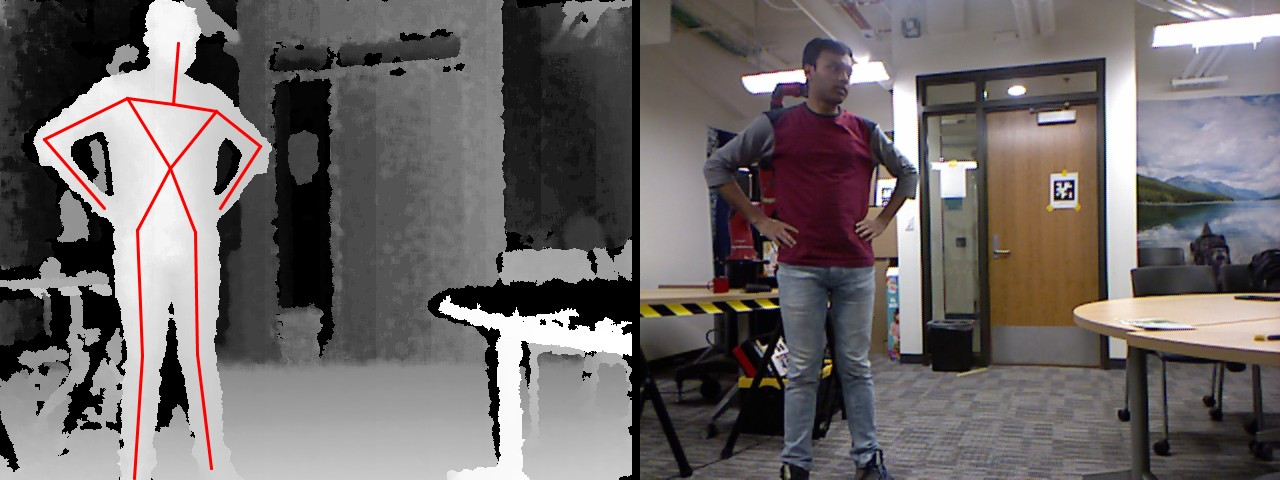
\includegraphics[scale=0.2]{sample_frame.jpg}
\caption{A sample frame captured from the Kinect sensor. Left: Raw depth image with 15-joint skeleton superimposed. Right: Raw RGB camera image.}
\label{fig:rawframe}
\end{figure}

\subsection{Data Collection}
\begin{figure}
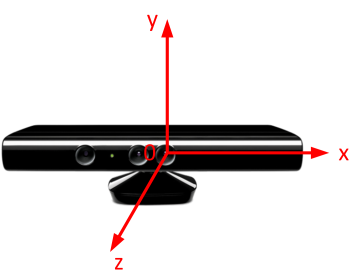
\includegraphics[scale=4]{kinect.png}
\caption{The Kinect camera frame.}
\label{fig:rawframe}
\end{figure}
We used the Microsoft Kinect 360 sensor and the \textit{SimpleOpenNI} library \cite{simpleopenni} to capture 3D joint coordinates (x, y, z) in the Kinect camera frame for a given person. Our \textit{Processing} script captures positions of 15 joints -- head, neck, torso, left shoulder, left elbow, left hand, right shoulder, right elbow, right hand, left hip, left knee, left foot, right hip, right knee, and right foot. Frame-by-frame joint positions and the associated frame timestamp relative to the beginning of capture were written to a JSON file. Simultaneous stereo-channel audio capture was also performed using \textit{Minim} \cite{minimlib}, a Java-based audio processing library, and saved to a WAV file.

Participants for data capture were asked to minimize iconic gestures (eg: pointing or mimicking) and exhibit primarily beat gestures, though a small percentage of pose frames do show iconic gestures which only adds noise to our dataset. This is a reasonable expectation to have from real-world datasets and asking participants to completely discard iconic gestures would make the recording seem unnatural. We do not segment out these iconic gestures.

Audio was recorded from the laptop microphone. Video frames were captured against a plain background and in the absence of natural light to minimize interference with the Kinect\textquotesingle s infrared sensor. Only a single voice (of the participant himself) was recorded. The recorded frames and audio were also captured to be as relevant as possible -- extraneous statements such as \textquotesingle can I start now?\textquotesingle  or  \textquotesingle let me know when you are ready\textquotesingle   were edited out later. Participants were asked to speak about a recent experience or share informational content -- for instance, one participant chose to talk about their recent experience at a restaurant, and another chose to discuss immigration policy for international students in the United States.

We collected approximately 30 minutes of training data spanning 6 different participants.

\subsection{Skeletal Data Processing}
Our dataset contains people of varying heights and, in general, different people exhibit different kinds of beat gestures. We also noticed that one data capture subject showed a lot of translational and rotational motion. In order to remove such variation across the dataset and to reduce dimensionality (to make speech-to-gesture modeling faster), we converted each frame\textquotesingle s 15-joint 3D coordinate representation (45 dimensions) to a 9-dimensional space of radian joint angles -- head\_neck\_torso, neck\_leftShoulder\_leftElbow, neck\_rightShoulder\_rightElbow, leftShoulder\_leftElbow\_leftHand, rightShoulder\_rightElbow\_rightHand, torso\_leftHip\_leftKnee, \\torso\_rightHip\_rightKnee, \\leftHip\_leftKnee\_leftFoot, and rightHip\_rightKnee\_rightFoot (the middle joint name represents angle vertex).

Angle between Joint 1, Vertex Joint, and Joint 3 was calculated as follows:\\
\begin{displaymath}
\arctan\left (\frac{\textbf{n} \cdot \left( \textbf{v1} \times \textbf{v2}\right )}{\textbf{v1} \cdot \textbf{v2}} \right ),
\end{displaymath}
where
\begin{displaymath}
\textbf{v1} = \textbf{joint\_1\_position} -  \textbf{vertex\_joint\_position},
\end{displaymath}
\begin{displaymath}
\textbf{v2} = \textbf{joint\_3\_position} -  \textbf{vertex\_joint\_position},
\end{displaymath}
and
\begin{displaymath}
\textbf{n} = \frac{\textbf{v1} \times \textbf{v2}}{\left \| \textbf{v1} \times \textbf{v2} \right \|}
\end{displaymath}\\
Angles are defined in the plane formed by the 2 vectors originating from the vertex joint. Additionally, cross product produces NaN values when all points are in the same line, but we do not need to worry about this because this is never the case with noisy real-world measurements.

\subsection{Base Poses}
\begin{figure}
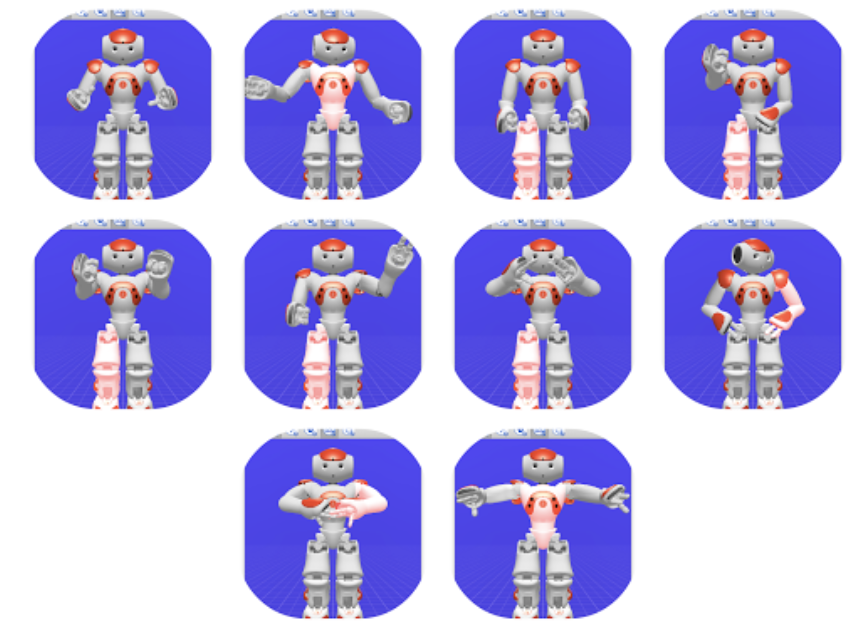
\includegraphics[scale=0.5]{poses.png}
\caption{10 base poses on the NAO robot.}
\label{fig:baseposes}
\end{figure}

To reduce the space of possible gestures as a way of simplifying our approach, we obtained a dataset of 10 stationary base poses. We chose these poses based on a browse through our original dataset to see which positions were most common among the human subjects who provided the data. We then find the closest (by Euclidean distance) base pose for each pose in the original dataset and label each original pose as being one of the 10 base poses. Recall that a pose is defined as a 9-dimensional vector of joint angles.

We predefine these poses on the NAO platform using the \textit{Aldebaran Choregraphe} software \cite{choregraphe}. Figure ~\ref{fig:baseposes} shows how these poses appear on the NAO robot, our chosen platform for experimentation.

\subsection{Audio Feature Extraction}
\begin{figure}
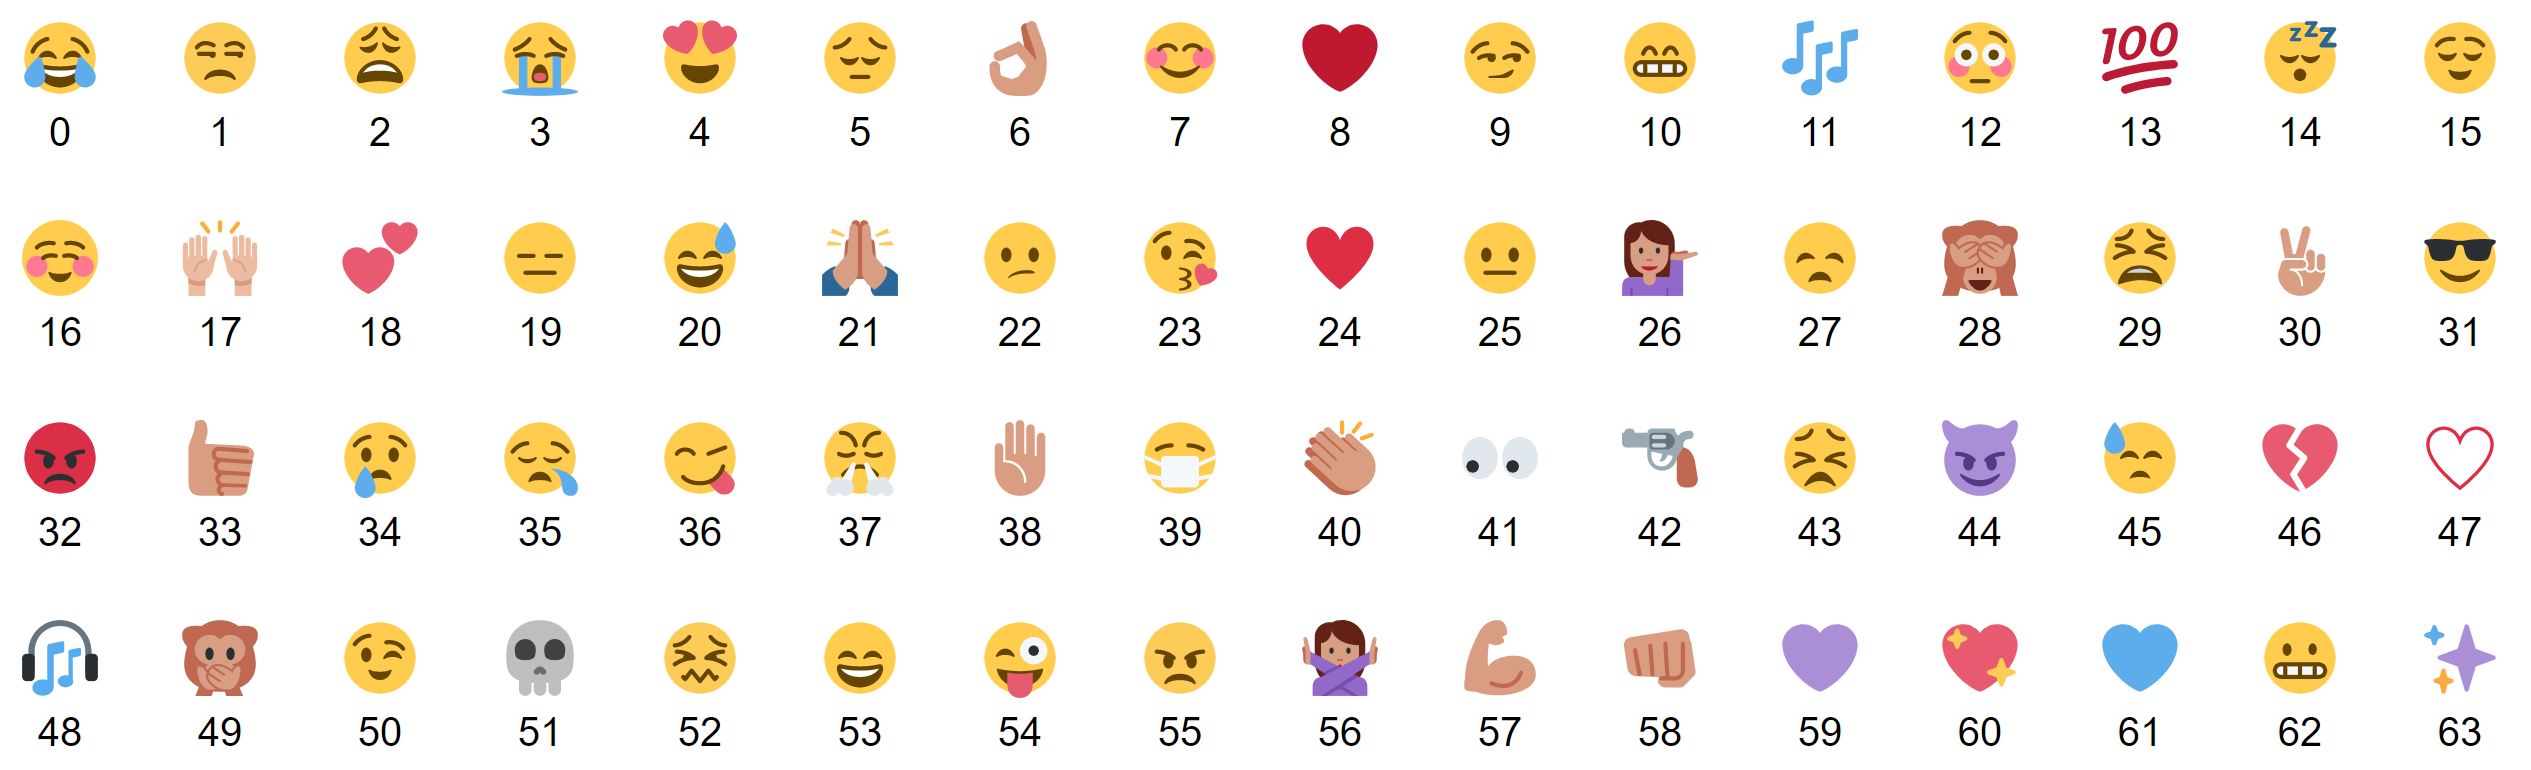
\includegraphics[scale=0.25]{emoji_overview.png}
\caption{Emojis and associated index labels \cite{deepmojipaper:3}.}
\label{fig:emojis}
\end{figure}

The stereo-channel audio file associated with a captured pose sequence is first converted to a mono-channel audio file because of the requirements set by the prosody extraction and speech-to-text utilities that we use. This mono-channel audio file is split into chunks based on a silence threshold -- in order for part of the waveform to be considered silent, it must be quieter than -50dBFS\footnote{dBFS = decibels relative to full scale. It is a unit of measurement for a digital signal\textquotesingle s amplitude. 0dBFS corresponds to the highest possible value for the amplitude.} for at least 1 second. These values were chosen based on trial-and-error and are loosely based on the assumption that humans don\textquotesingle t use beat gestures when they are quiet, which comes from our observation of the dataset. We tested several values for these 2 variables and these values, based on manual inspection, seemed to yield the best balance between getting most of the relevant information and not making the chunk size too small so as to make it unusable for emotion feature extraction. Audio chunks less than 2 seconds in length were also discarded because they do not contain any significant information for emotion feature extraction.

For each audio chunk, we extracted a 13-element prosody vector\footnote{Described here: https://github.com/jcvasquezc/DisVoice/blob/master/prosody/README.md} and a 64-element emotion vector.

The 13-element prosody feature vector was extracted using the DisVoice framework \cite{disvoice}, initially developed to characterize voice disorders. All 13 static features can be categorized into one of 3 characteristics of speech that define prosody: duration, fundamental frequency, and energy.

The 64-element emotion feature vector was derived using the DeepMoji framework. DeepMoji is a deep learning model that returns the top-5 emojis (out of a total of 64), ranked in descending order by probability scores, and their labels associated with a given input text. We used torchMoji \cite{torchmoji}, a pyTorch implementation of the DeepMoji model, for programmatic ease. The model essentially adds more dimensions to sentiment analysis by pushing it beyond the simple binary positive/negative classification. Emojis offer a rich space of human emotional expression and the model\textquotesingle s tweet-based training captures a lot of variation in human emotion from a wide spectrum of the population.

We convert each of the top-5 labels into a 64-element one-hot encoding and squash the 5 one-hot encodings into a single 64-element vector that contains 5 1s. We used the \textit{Google Cloud API} \cite{gcloud} to convert audio to text which is then fed into torchMoji. We realize this may induce errors into our system as automatic speech-to-text is not perfect, especially for users with heavy accents, but we found that such an approach works for the most part and is obviously more scalable than manual transcription. In the future, it might be helpful to do a side-by-side comparison of this approach with the manual method and see how it affects accuracies of the speech-to-gesture model and the eventual subjective evaluation of robot gesture playback.

\subsection{Final Dataset}

Our final dataset consists of approximately 12,000 samples, 64 emotion features, 13 prosody features, and 9 pose angles associated with a given audio feature.


\section{Speech-to-Gesture Model}
We tested 3 machine learning methods for mapping input audio features to output joint angles: k-Nearest Neighbors (kNN), Logistic Regression, and Long-Short Term Memory (LSTM).

We tested 3 input feature types -- 64-element one-hot encoding of emotion features extracted from text, 13-element prosody vector (scaled to range [0, 1] and NaN values replaced by zeros) extracted from audio, and a 77-element combined feature vector which is a concatenation of the 64-element emotion feature vector and the 13-element prosody feature vector.

We train on the data captured from the first 5 participants and test on the last participant's data.

\subsection{k-Nearest Neighbors}
We use the default kNN classifier provided by \textit{scikit-learn} \cite{sklearn} with k=5 and points in a given neighborhood weighted uniformly. This classifier outputs a base pose index.

\subsection{Logistic Regression}
We use the default Logistic Regression classifier provided by \textit{scikit-learn} with L2 penalty, stopping criteria tolerance of 0.0001, and 100 maximum iterations. This classifier outputs a base pose index.

\subsection{LSTM}
This model is a simple LSTM model with audio feature vectors as inputs and joint angles as outputs. Dropout is set to 0.2 to make the network more robust. We use the Adam optimizer to minimize our loss function.

We noticed that adding a fully-connected layer after the LSTM layer bumps up the overall accuracy to almost 100\%. This, combined with the fact that our dataset is small-scale, made us believe our model was prone to overfitting, so we removed the Dense layer. 

The angle loss function is defined as the Euclidean distance between the true angle values and the predicted angle values:
\begin{displaymath}
angle\_loss = \sqrt{\sum_{i=1}^n (angle\_true_i - angle\_pred_i)^2}
\end{displaymath}
\section{Experimental Setup}
In addition to doing an objective, accuracy-based evaluation for our speech-to-gesture models, we also do a subjective evaluation of the generated gestures.

We split our subjective evaluation across 3 control and 3 experimental conditions as follows:
\begin{enumerate}
\item \textit{Control}: Human recording played back on the robot
\item \textit{Control}: No gestures
\item \textit{Control}: Random gestures
\item \textit{Experimental}: Prosody-based gestures
\item \textit{Experimental}: Emotion-based gestures
\item \textit{Experimental}: Prosody+emotion-based gestures
\end{enumerate}
\subsection{Sequence Generation}
We used the highest-accuracy yielding method for each input feature type to generate final sequences for playback on the robot -- kNN for emotion and prosody features, and logistic regression for combined features.

We use audio from the last participant to generate gesture sequences. This dataset is not used in training our speech-to-gesture models.

We used the NAO robot as our model in the \textit{Choregraphe} software. The NAO robot is humanoid in nature and therefore makes mapping human gestures onto it quite trivial. Gesture sequences were generated slightly differently for each experimental condition:
\begin{itemize}
\item Human playback -- Our original dataset shows that one audio chunk can correspond to multiple pose frames. Additionally, in order to ensure smooth playback in \textit{Choregraphe}, we hard-coded the duration each pose should take to execute to 1 second. Because the total number of pose frames in the original dataset corresponding to a given audio file is not necessarily equal to the length of the audio file (in seconds), we had to sample frames sequentially for each audio chunk. The number of frames sampled uniformly at random from each audio chunk was equal to the length of that audio chunk (in seconds). This process was done for each audio chunk in a given audio file and poses were concatenated and saved to a .txt file, which can then be read in by \textit{Choregraphe}.
\item No gestures -- A list of 2s was written to a .txt file as the sequence of poses. The length of this list was the length of the associated audio file in seconds. Pose 2 from our list of base poses (indexed by 0) is a neutral standing posture with arms on either side and legs shoulder width apart (see third pose in top row in Figure ~\ref{fig:baseposes}).
\item Random gestures -- A list of integers in range [0, 9] corresponding to base pose indices was generated by selecting poses uniformly at random. The length of this list was the length of the associated audio file in seconds.
\item Emotion-, Prosody-, Combined feature-based gestures -- We take the previously unseen audio file and split it into chunks of 5 seconds. Audio features are computed for each chunk and fed into our chosen speech-to-gesture model as many times as there are seconds in the given audio file chunk (here, 5, with some variable number of seconds at the end because not all audio files are of length divisible by 5). This is a severe limitation in our crude design since the same audio features being fed into the model output the same pose index, which made the output sequence "[feel] like a total disconnect between what was being said and [the robot\textquotesingle s] motions," as one survey participant noted.

\end{itemize}
\subsection{Robot Playback}
Mapping of human joint positions to those of the NAO robot was a challenging task. There are an infinite number of poses and there are a number of factors to consider when constructing this mapping. We simplified this problem by restricting and confining to 10 most frequently occurring poses. These 10 base poses were then predefined in \textit{Choregraphe}. The Python script we created takes as input a .txt file that contains a list of pose indices that are designed to play for the exact length of time as the audio clip. When playing back poses on the robot, \textit{Choregraphe} automatically interpolates between these pre-defined poses based on whatever order is generated by our speech-to-gesture model. Audio is simultaneously played from disk and our sequence generation mechanism guarantees the synchronization of audio and video.

\subsection{Setup}
\begin{figure}
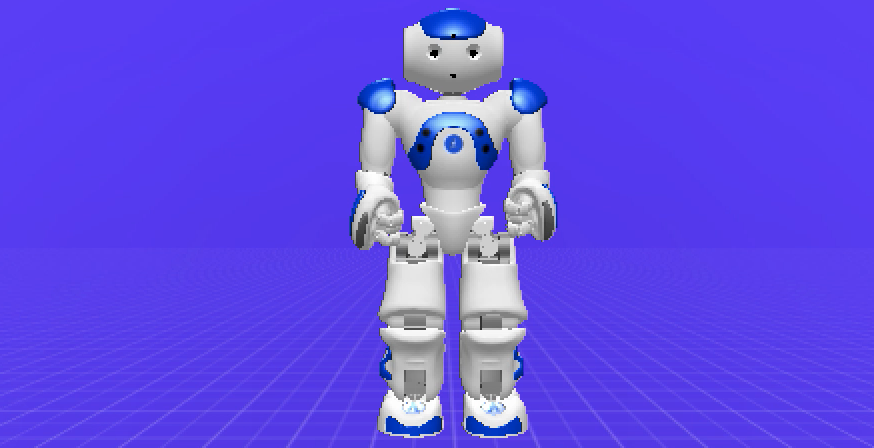
\includegraphics[scale=0.6]{final_frame.png}
\caption{A frame from a typical video shown to survey participants.}
\label{fig:frameshown}
\end{figure}
Participants are asked to pick one video at random from a total of 6 -- one for each experimental condition. All videos are accompanied by the same speech. Videos are screencasts of the simulation environment within \textit{Choregraphe} of the NAO robot against a blue background (see Figure ~\ref{fig:frameshown} for a video frame). Videos are 2 minutes in length. After watching the assigned video, participants are asked to fill out a subjective evaluation that contains 8 5-point Likert scale statements [1=strongly disagree, 5=strongly agree]. Each statement is followed by an optional space where participants can respond in free-form regarding their thoughts about the statement in relation to the video they just watched. We also provide a free-response section at the end of the evaluation for any aspects that weren\textquotesingle t covered by the questions. We used the following statements:
\begin{enumerate}
\item Movements were timed appropriately.
\item The robot was engaging.
\item Motions were consistent with speech.
\item Movements appeared natural and human-like.
\item I perceive the robot in a friendly, positive light.
\item The robot's movements were seamless and fluid.
\item The robot seemed relatable.
\item I can see myself engaging in long-term conversation with this robot.
\end{enumerate}

Statements (1) and (3) were borrowed from \cite{levine:2}.

Note that there is redundancy among these statements to ensure consistent responses.
\subsection{Hypothesis}
We hypothesize that humans will order each of our 6 test conditions in decreasing order of gesture naturalness as follows: human playback, combined prosody+emotion-based gestures, either prosody- or emotion-based gestures, and either random or no gestures.

\section{Results and Discussion}
\begin{figure}
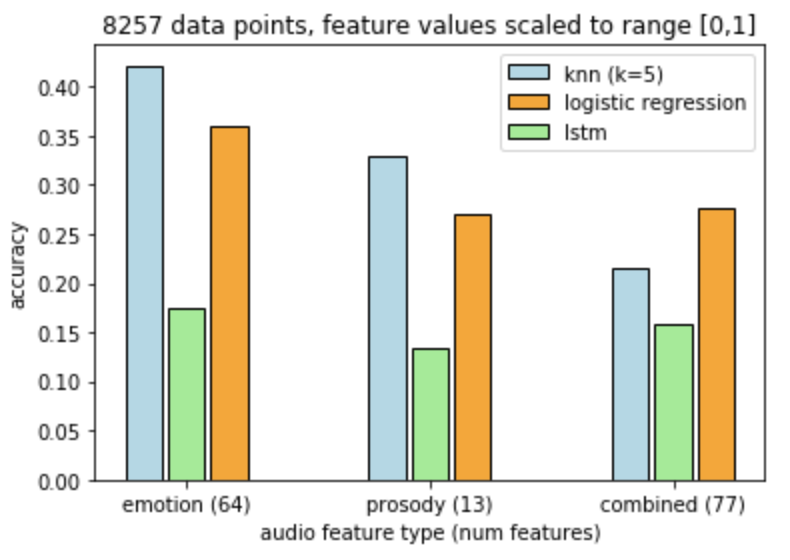
\includegraphics[scale=0.6]{results_new2.png}
\caption{A bar chart showing the accuracies of our machine learning models.}
\label{fig:acc}
\end{figure}

\begin{figure}
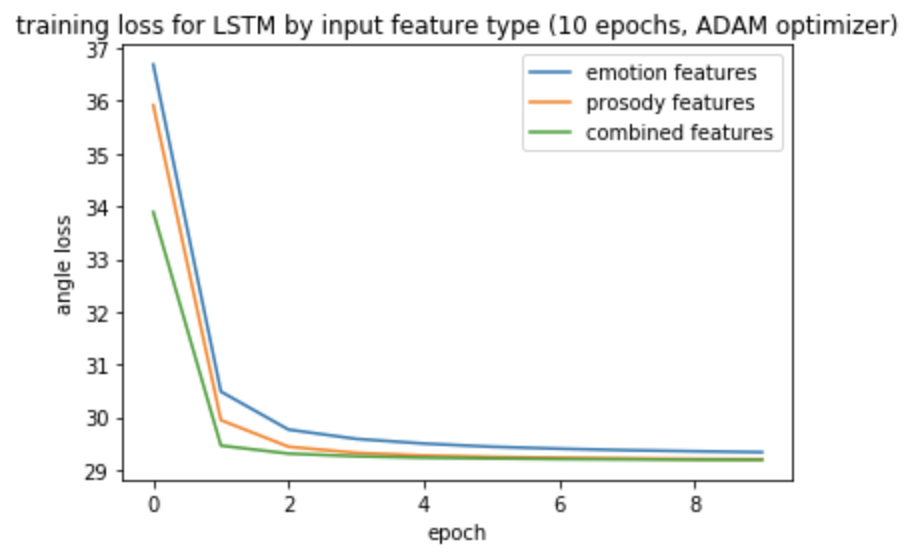
\includegraphics[scale=0.6]{loss.png}
\caption{Line plots showing the loss values for our LSTM model.}
\label{fig:loss}
\end{figure}

\begin{figure}
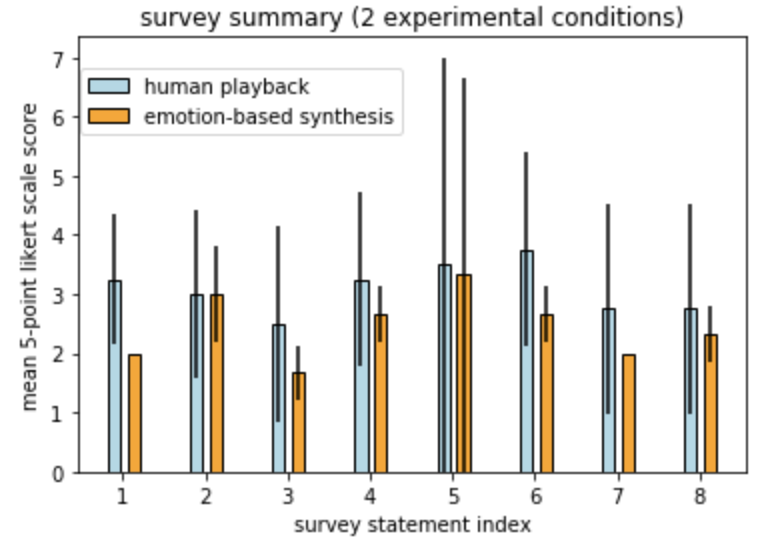
\includegraphics[scale=0.6]{survey1.png}
\caption{A bar chart (with error bars for 1 standard deviation) summarizing our survey results for 7 participants.}
\label{fig:survey}
\end{figure}

\subsection{Objective Evaluation for Speech-to-Gesture Models}
Figure ~\ref{fig:acc} shows the test accuracies for the three machine learning models that we tried for each of the 3 input feature types. Note that feature values are rescaled to range [0, 1].

kNN performs better overall for the emotion and prosody scenarios, but worse than logistic regression for the combined feature input. LSTM consistently performs poorly for all 3 input feature types. We expected LSTM to perform the best out of all three because it is specifically designed for sequence learning, however we suspect it performed poorly due to lack of data or lack of appropriate parameter tuning. It was also interesting to observe that despite feeding in different feature vectors, the output of our LSTM model was more often than not the same pose index.

Still, all our models perform far better than the baseline accuracy of 10\%. This baseline is 10\% because we have 10 base poses.
\subsection{Subjective Evaluation for Pose Sequence Playback on Robot}
We conducted an informal survey to test our hypothesis, however we were only able to obtain data for 2 conditions -- emotion-driven synthesis and human playback -- from 7 participants in total.

Figure ~\ref{fig:survey} summarizes our survey results for the 2 out of 6 experimental conditions. Note how the scores for human playback are consistently higher than the scores for emotion-based synthesis. Therefore, participants\textquotesingle views confirmed the relative ranking of the two methods, as we hypothesized.

On the contrary, free-response feedback is more mixed and borderline inconclusive. While some participants reported that human replay seemed "choppy and random" and that they "weren\textquotesingle t sure what the robot was trying to communicate," others reported the robot as being "expressive."

Free-response feedback regarding emotion-driven synthesis was consistently reported as being "out of sync" and motions as being "too far apart."

One participant reported not being able to understand the audio. This is quality issue and can be fixed easily. 

Some participants weren\textquotesingle t sure what the robot motions were trying to communicate. This could be due to the limited variability in robot poses, poor timing of motions, or us as experimenters being unclear in communicating the purpose of this experiment to the participants.

In the future, we can improve upon our evaluation procedure by assigning random videos to participants ourselves to ensure complete coverage of our experimental conditions.

\section{Conclusion}
\subsection{Summary}
We implemented and evaluated a model for converting human speech to robot gestures. kNN model seemed to yield the best results even though we expected LSTM to do better. We also designed a mapping from human joints to robot joints. We hypothesized that humans will order each of our 6 test conditions in decreasing order of naturalness as follows: human playback, combined prosody+emotion-based gestures, either prosody- or emotion-based gestures, and either random or no gestures. We conducted an informal survey to test our hypothesis, however we were only able to obtain data for 2 conditions -- emotion-driven synthesis and human playback -- and people's views confirmed the relative ranking of the two methods.

\subsection{Limitations and Future Work}
There are several limitations to the approach we presented here. And certainly, these limitations can serve as valid avenues for future work.

First, we restrict our gesture generation to 10 base poses. This severely limits the variability of poses a robot can exhibit. A simple way to overcome this limitation would be to have a clustering algorithm automatic identify these base poses, which should result in a greater variety that captures both variations in poses on an individual level and variations in poses across different people.

Second, our classifiers don\textquotesingle t yield accuracies of more than 50\%. More data and better parameter tuning could boost the overall accuracy of our models. An overlapping window-based approach combined with traditional machine learning models could also help better capture sequential dependencies between data points.

Third, doing sequence generation in realtime would make our system more attractive. Not only that, but also coming up with a better scheme to do sequence generation than simply playing a given pose based on the duration of the audio chunk would help make the generated gestures more natural and varied.

Fourth, it would be useful to develop a generic human-to-robot embodiment mapping interface that works regardless the DoF configurations of the robot in consideration. We worked with the NAO robot which is humanoid in terms of degrees of freedom (DoFs), but our system will be more attractive if it can generalize to different robot types.

Fifth, it would be interesting to see how beat gestures vary across different humans. We can record the same speech from different participants and analyze body language variations. This should help us develop a more generalizable approach to robot gesture generation.

Sixth, controlling pose speed is also a major challenge. In our current approach we set motor torques to 75\% of the full value, but being able to control this algorithmically will give the robot more flexibility in expressing gestures. Running the experiment on a real robot would also be useful, not only to see if it works as it does in simulation but also to investigate how the physical presence of a robot impacts the naturalness of human-robot interaction.

Overall, we believe it is important to give robots the ability to generate human-like body language in order to make human-robot interactions more fluid and dynamic. There remains a lot of work to be done in building such a system and making it robust, generalizable, and scalable for real-world applications.
\begin{acks}
We would like to thank Prof. Brad Hayes for his constant feedback and mentorship regarding project design and direction. We would also like to thank our data collection participants for their time and the survey participants for providing free-response feedback which gave us ideas on what can be improved in future iterations of our system.
\end{acks}

\bibliographystyle{ACM-Reference-Format}
\bibliography{sample-bibliography}

\end{document}
